\section{Array\-List\-Enumeration Class Reference}
\label{classArrayListEnumeration}\index{ArrayListEnumeration@{ArrayListEnumeration}}
An implementation of the Array\-Enumaration based on the Array\-List class.  


{\tt \#include $<$Array\-List\-Enumeration.h$>$}

Inheritance diagram for Array\-List\-Enumeration:\begin{figure}[H]
\begin{center}
\leavevmode
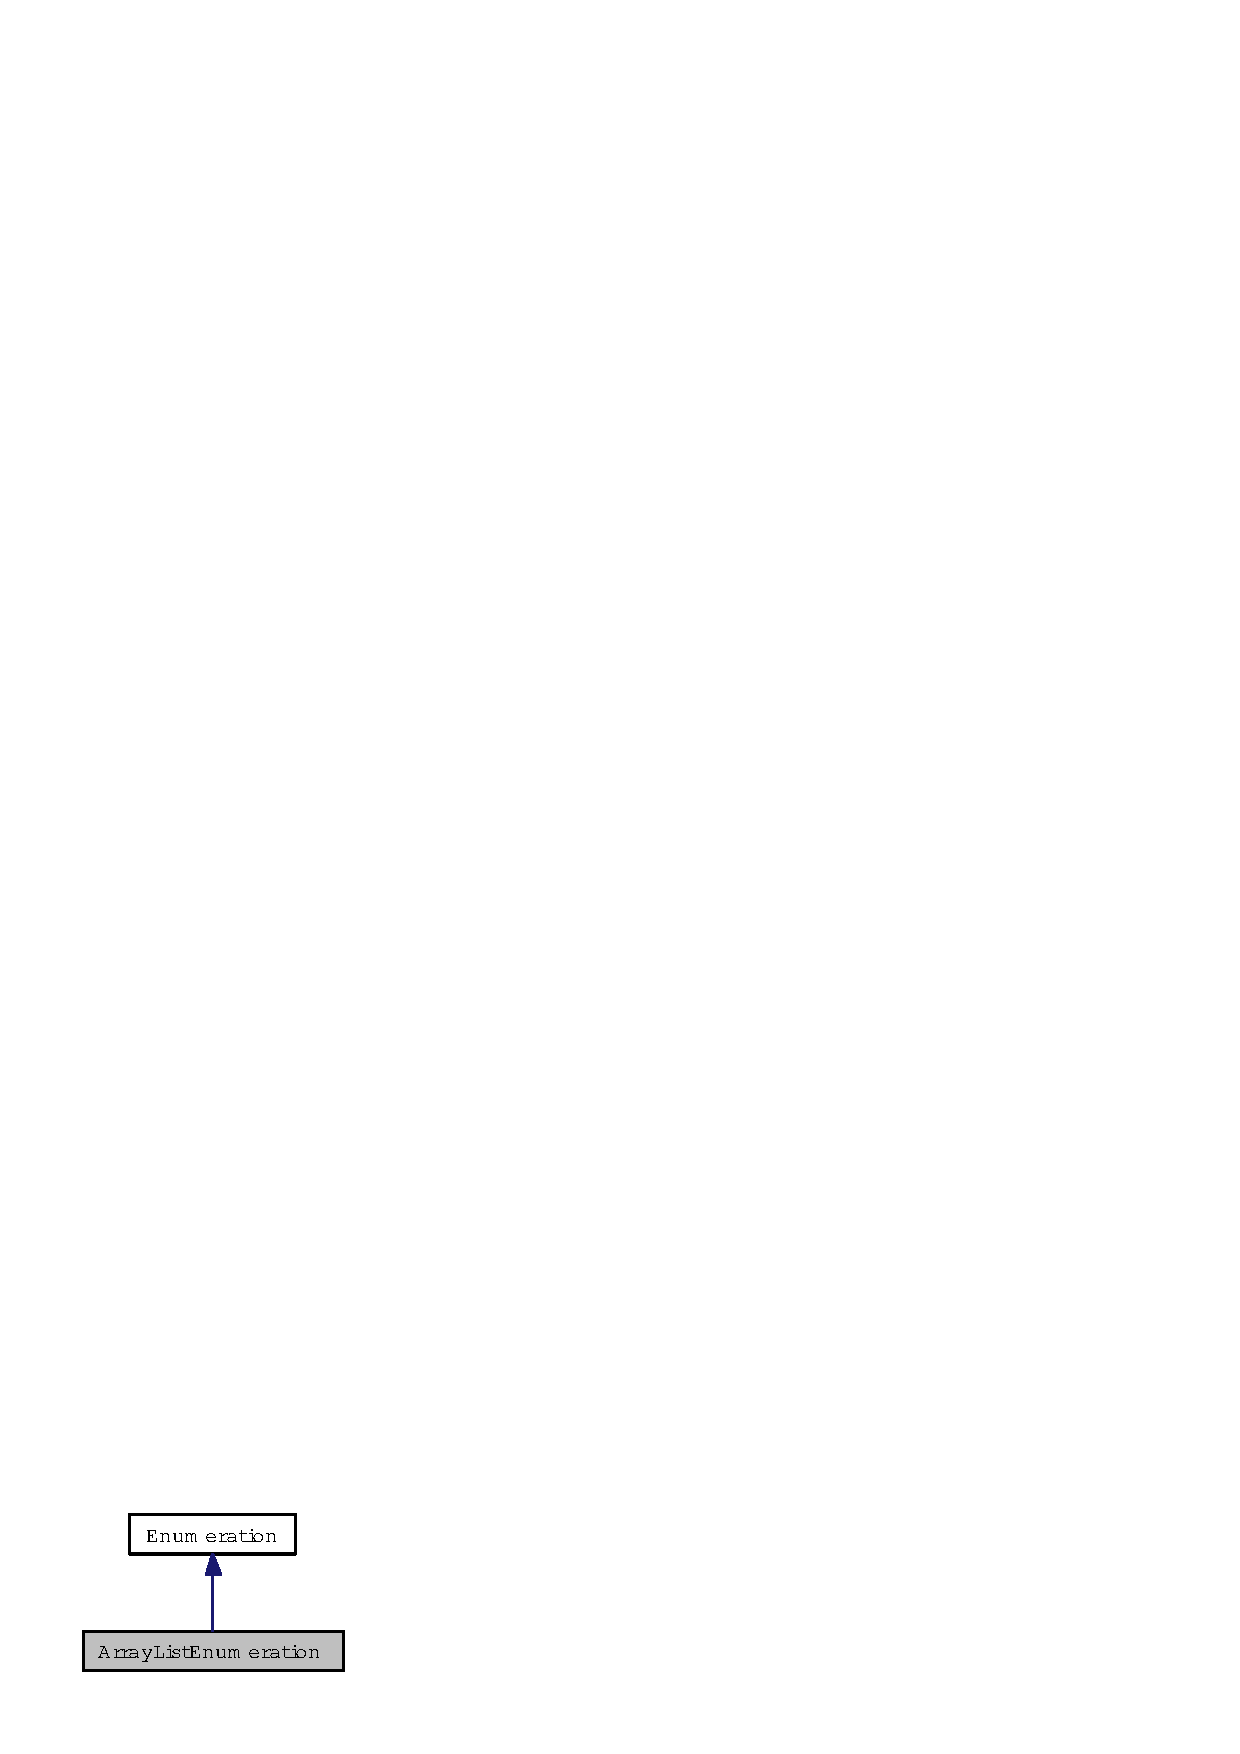
\includegraphics[width=84pt]{classArrayListEnumeration__inherit__graph}
\end{center}
\end{figure}
Collaboration diagram for Array\-List\-Enumeration:\begin{figure}[H]
\begin{center}
\leavevmode
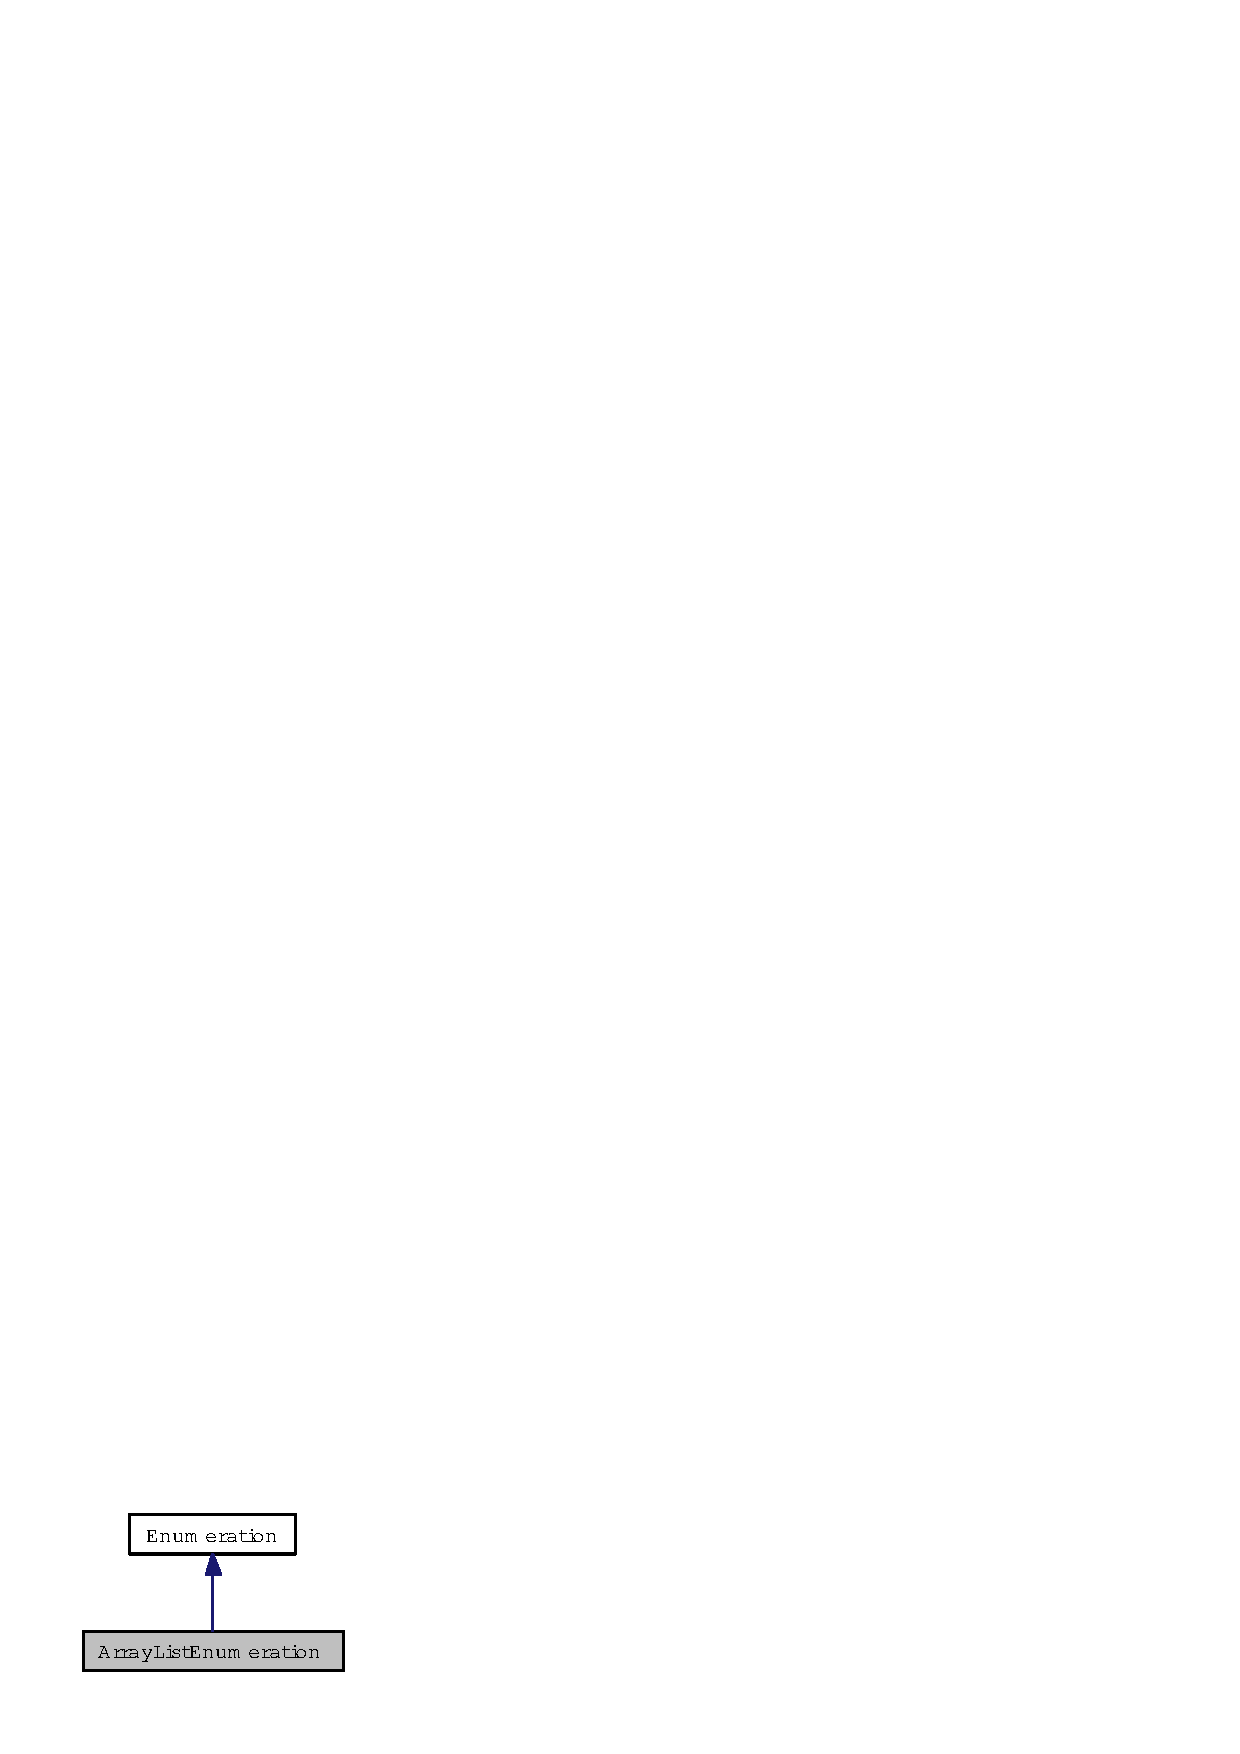
\includegraphics[width=84pt]{classArrayListEnumeration__coll__graph}
\end{center}
\end{figure}
\subsection*{Public Member Functions}
\begin{CompactItemize}
\item 
\textbf{Array\-List\-Enumeration} (const Array\-List \&l)\label{classArrayListEnumeration_ab05789262170aa2c3df3a895b18540f}

\item 
bool {\bf has\-More\-Element} () const\label{classArrayListEnumeration_39325e1320707c1d90524ea1643d32c1}

\begin{CompactList}\small\item\em Return true if there are more elements in the enumeration. \item\end{CompactList}\item 
Array\-Element $\ast$ {\bf get\-Next\-Element} ()\label{classArrayListEnumeration_46c03d96b85c61cd3338646d57da5e8c}

\begin{CompactList}\small\item\em Return the next element. \item\end{CompactList}\end{CompactItemize}


\subsection{Detailed Description}
An implementation of the Array\-Enumaration based on the Array\-List class. 



The documentation for this class was generated from the following file:\begin{CompactItemize}
\item 
src/include/common/base/util/Array\-List\-Enumeration.h\end{CompactItemize}
